\documentclass[11pt,a4paper]{report}
\usepackage[textwidth=37em,vmargin=30mm]{geometry}
\usepackage{calc,xunicode,amsmath,amssymb,paralist,enumitem,tabu,booktabs,datetime2,xeCJK,xeCJKfntef,listings}
\usepackage{tocloft,fancyhdr,tcolorbox,xcolor,graphicx,eso-pic,xltxtra,xelatexemoji}

\newcommand{\envyear}[0]{2025}
\newcommand{\envdatestr}[0]{2025-08-27}
\newcommand{\envfinaldir}[0]{webdb/2025/20250827/final}

\usepackage[hidelinks]{hyperref}
\hypersetup{
    colorlinks=false,
    pdfpagemode=FullScreen,
    pdftitle={Web Digest - \envdatestr}
}

\setlength{\cftbeforechapskip}{10pt}
\renewcommand{\cftchapfont}{\rmfamily\bfseries\large\raggedright}
\setlength{\cftbeforesecskip}{2pt}
\renewcommand{\cftsecfont}{\sffamily\small\raggedright}

\setdefaultleftmargin{2em}{2em}{1em}{1em}{1em}{1em}

\usepackage{xeCJK,xeCJKfntef}
\xeCJKsetup{PunctStyle=plain,RubberPunctSkip=false,CJKglue=\strut\hskip 0pt plus 0.1em minus 0.05em,CJKecglue=\strut\hskip 0.22em plus 0.2em}
\XeTeXlinebreaklocale "zh"
\XeTeXlinebreakskip = 0pt


\setmainfont{Brygada 1918}
\setromanfont{Brygada 1918}
\setsansfont{IBM Plex Sans}
\setmonofont{JetBrains Mono NL}
\setCJKmainfont{Noto Serif CJK SC}
\setCJKromanfont{Noto Serif CJK SC}
\setCJKsansfont{Noto Sans CJK SC}
\setCJKmonofont{Noto Sans CJK SC}

\setlength{\parindent}{0pt}
\setlength{\parskip}{8pt}
\linespread{1.15}

\lstset{
	basicstyle=\ttfamily\footnotesize,
	numbersep=5pt,
	backgroundcolor=\color{black!5},
	showspaces=false,
	showstringspaces=false,
	showtabs=false,
	tabsize=2,
	captionpos=b,
	breaklines=true,
	breakatwhitespace=true,
	breakautoindent=true,
	linewidth=\textwidth
}






\newcommand{\coverpic}[2]{
    % argv: itemurl, authorname
    Cover photo by #2~~(\href{#1}{#1})
}
\newcommand{\makeheader}[0]{
    \begin{titlepage}
        % \newgeometry{hmargin=15mm,tmargin=21mm,bmargin=12mm}
        \begin{center}
            
            \rmfamily\scshape
            \fontspec{BaskervilleF}
            \fontspec{Old Standard}
            \fontsize{59pt}{70pt}\selectfont
            WEB\hfill DIGEST
            
            \vfill
            % \vskip 30pt
            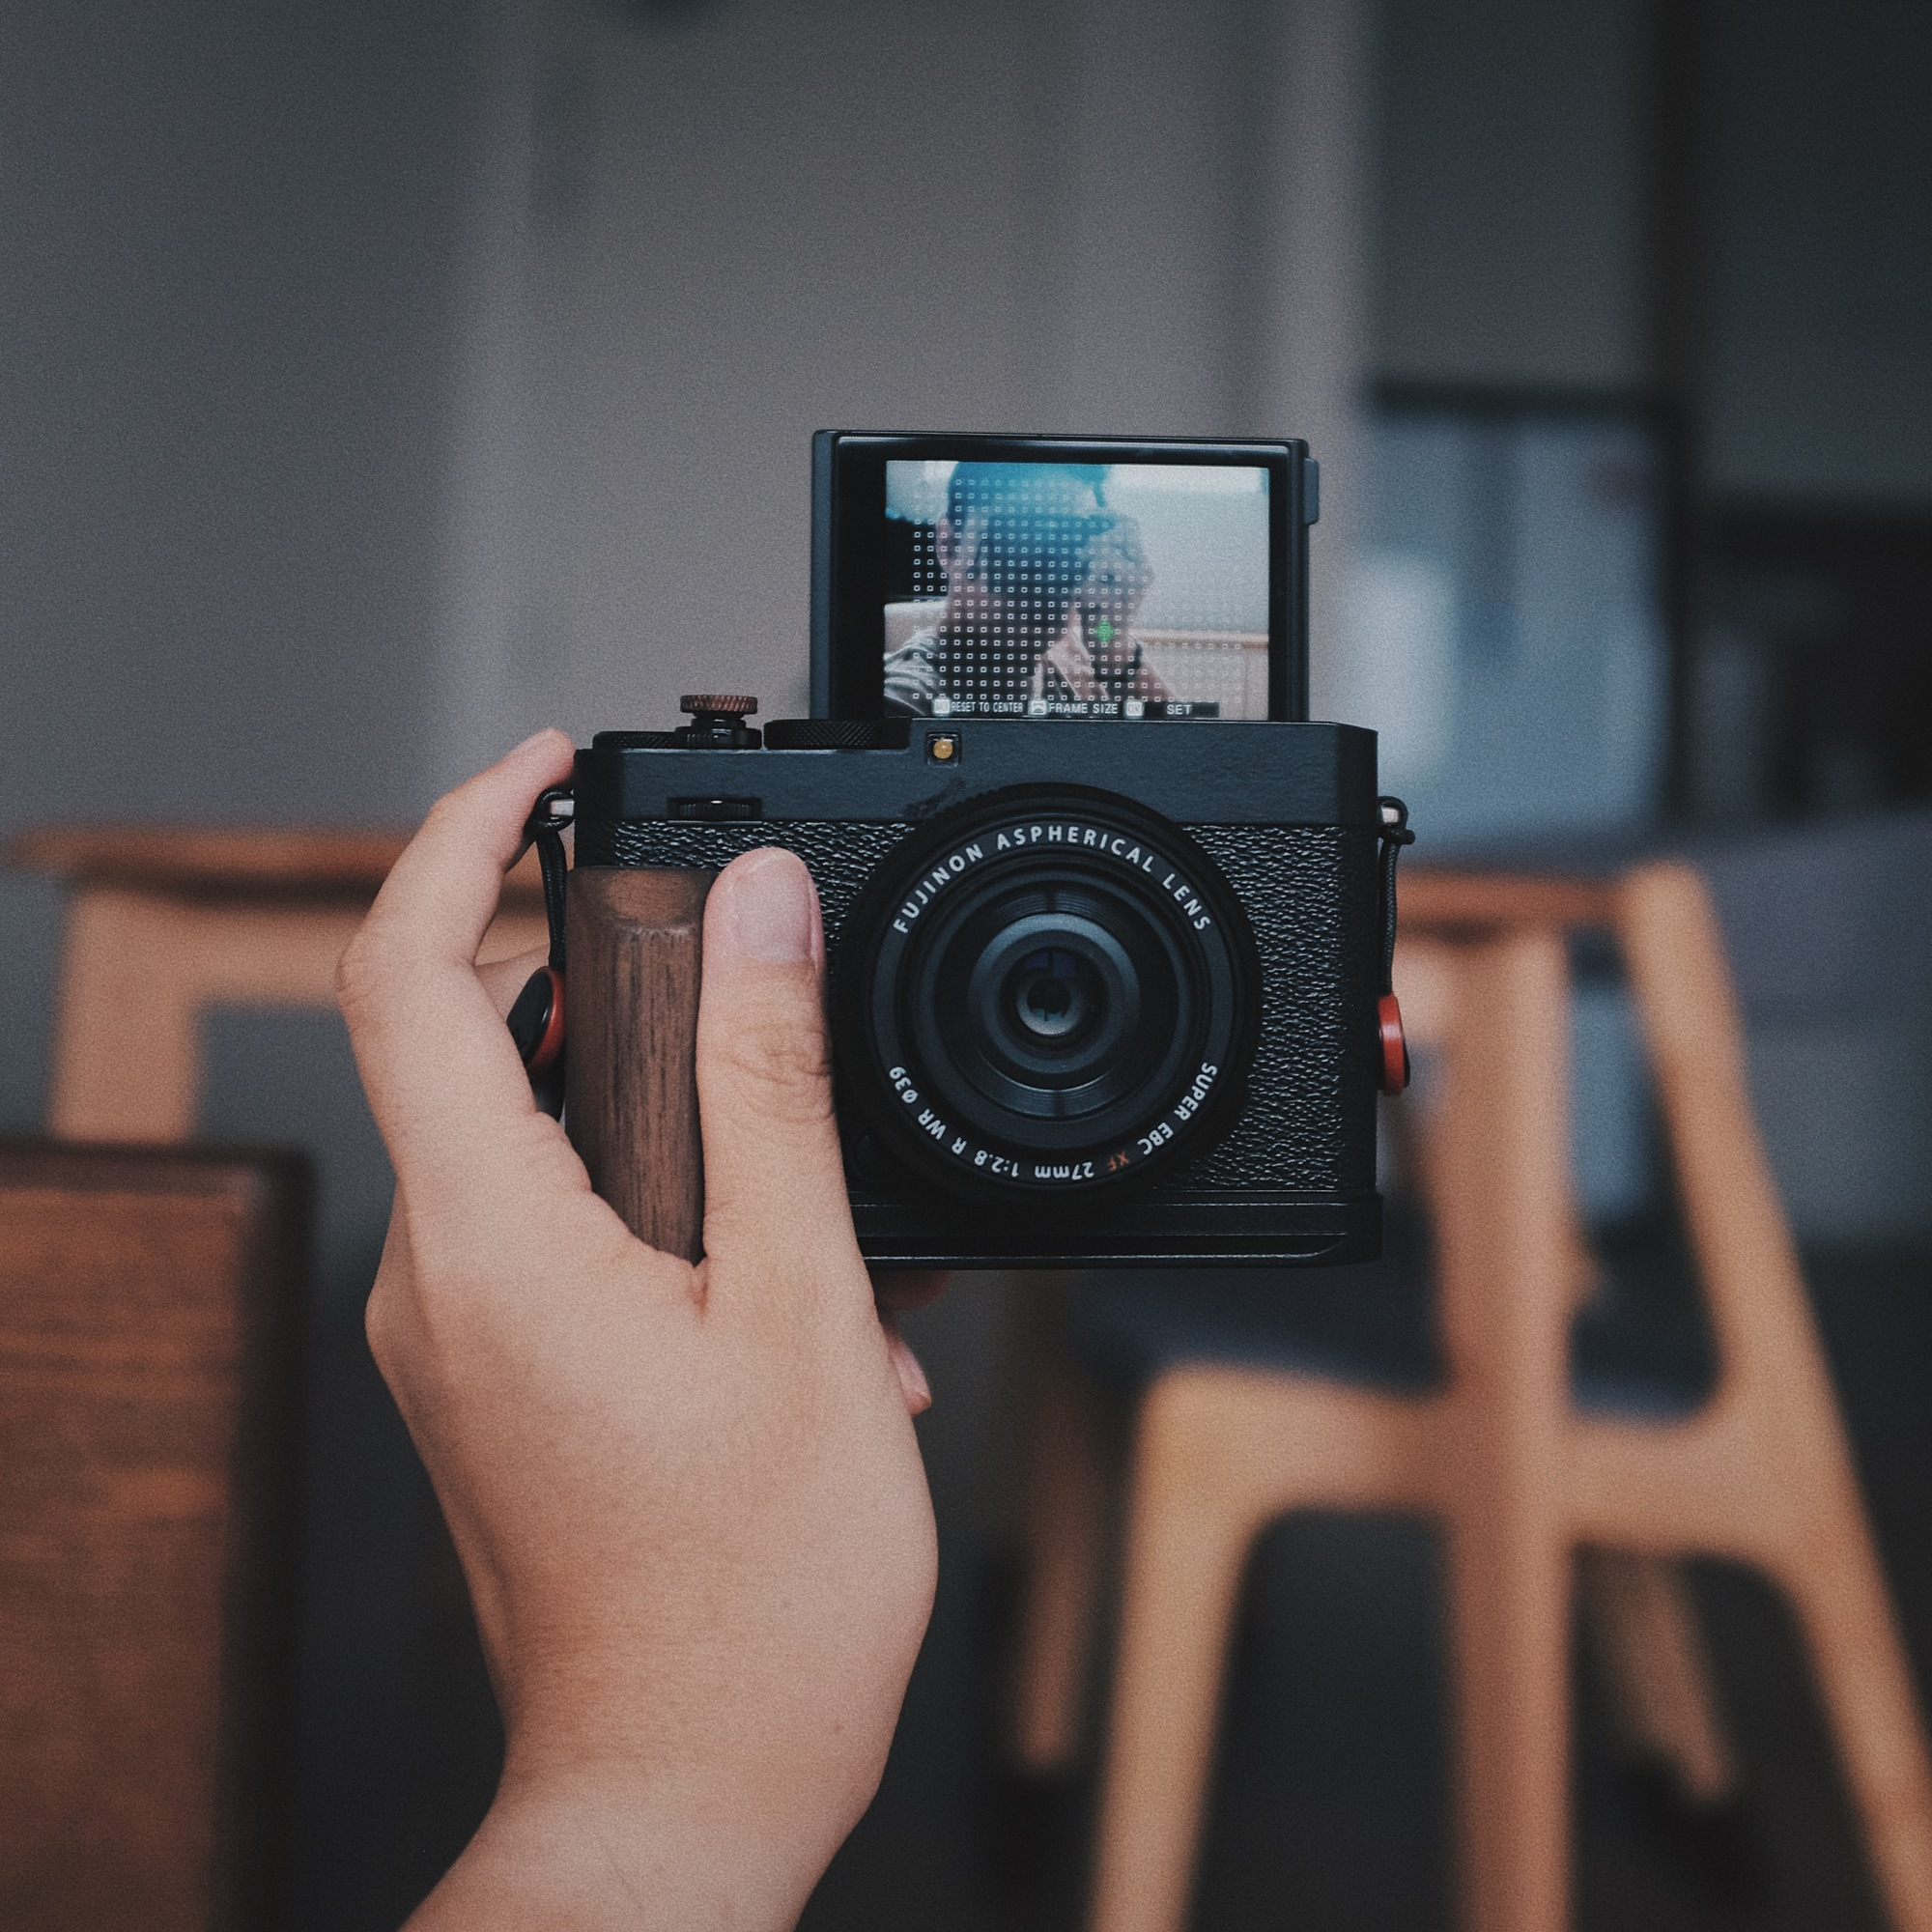
\includegraphics[width=\linewidth]{\envfinaldir/coverpic-prod.jpg}\par
            % \vskip 30pt
            \vfill

            \normalsize\rmfamily\scshape
            \copyright{} The Web Digest Project \hfill\large \envdatestr
        \end{center}
    \end{titlepage}
    % \restoregeometry
}
\newcommand{\simplehref}[1]{%
    \textcolor{blue!80!green}{\href{#1}{#1}}%
}
\renewcommand{\contentsname}{\center\Huge\sffamily\bfseries Contents\par\vskip 20pt}
\newcounter{ipartcounter}
\setcounter{ipartcounter}{0}
\newcommand{\ipart}[1]{
    % \vskip 20pt
    \clearpage
    \stepcounter{ipartcounter}
    \phantomsection
    \addcontentsline{toc}{chapter}{#1}
    % \begin{center}
    %     \Huge
    %     \sffamily\bfseries
    %     #1
    % \end{center}
    % \vskip 20pt plus 7pt
}
\newcounter{ichaptercounter}
\setcounter{ichaptercounter}{0}
\newcommand{\ichapter}[1]{
    % \vskip 20pt
    \clearpage
    \stepcounter{ichaptercounter}
    \phantomsection
    \addcontentsline{toc}{section}{\numberline{\arabic{ichaptercounter}}#1}
    \begin{center}
        \Huge
        \sffamily\bfseries
        #1
    \end{center}
    \vskip 20pt plus 7pt
}
\newcommand{\entrytitlefont}[1]{\subsection*{\raggedright\Large\sffamily\bfseries#1}}
\newcommand{\entryitemGeneric}[2]{
    % argv: title, url
    \parbox{\linewidth}{
        \entrytitlefont{#1}\par\vskip 5pt
        \footnotesize\ttfamily\mdseries
        \simplehref{#2}
    }\vskip 11pt plus 11pt minus 1pt
}
\newcommand{\entryitemGithub}[3]{
    % argv: title, url, desc
    \parbox{\linewidth}{
        \entrytitlefont{#1}\par\vskip 5pt
        \footnotesize\ttfamily\mdseries
        \simplehref{#2}\par\vskip 5pt
        \small\rmfamily\mdseries#3
    }\vskip 11pt plus 11pt minus 1pt
}
\newcommand{\entryitemAp}[3]{
    % argv: title, url, desc
    \parbox{\linewidth}{
        \entrytitlefont{#1}\par\vskip 5pt
        \footnotesize\ttfamily\mdseries
        \simplehref{#2}\par\vskip 5pt
        \small\rmfamily\mdseries#3
    }\vskip 11pt plus 11pt minus 1pt
}
\newcommand{\entryitemHackernews}[3]{
    % argv: title, hnurl, rawurl
    % \parbox{\linewidth}{
    %     \entrytitlefont{#1}\par\vskip 5pt
    %     \footnotesize\ttfamily\mdseries
    %     \simplehref{#3}\par
    %     \textcolor{black!50}{\href{#2}{#2}}
    % }\vskip 11pt plus 11pt minus 1pt
    \begin{minipage}{\linewidth}
            \entrytitlefont{#1}\par\vskip 5pt
            \footnotesize\ttfamily\mdseries
            \simplehref{#3}\par
            \textcolor{black!50}{\href{#2}{#2}}
    \end{minipage}\par\vskip 11pt plus 11pt minus 1pt
}







\begin{document}

\makeheader

\tableofcontents\clearpage




\ipart{Developers}
\ichapter{Hacker News}
\entryitemTwoLinks{GNU Artanis – A fast web application framework for Scheme}{https://news.ycombinator.com/item?id=45031673}{https://artanis.dev/index.html}

\entryitemTwoLinks{What happens when ambassadors are summoned by the host country?}{https://news.ycombinator.com/item?id=45031496}{https://politics.stackexchange.com/questions/93401/what-happens-when-ambassadors-are-summoned-by-the-foreign-ministry-of-their-host}

\entryitemTwoLinks{Claude for Chrome}{https://news.ycombinator.com/item?id=45030760}{https://www.anthropic.com/news/claude-for-chrome}

\entryitemTwoLinks{Why do people keep writing about the imaginary compound Cr2Gr2Te6?}{https://news.ycombinator.com/item?id=45030144}{https://www.righto.com/2025/08/Cr2Ge2Te6-not-Cr2Gr2Te6.html}

\entryitemTwoLinks{Michigan Supreme Court: Unrestricted phone searches violate Fourth Amendment}{https://news.ycombinator.com/item?id=45029764}{https://reclaimthenet.org/michigan-supreme-court-rules-phone-search-warrants-must-be-specific}

\entryitemTwoLinks{We regret but have to temporary suspend the shipments to USA}{https://news.ycombinator.com/item?id=45029579}{https://olimex.wordpress.com/2025/08/26/we-regret-but-have-to-temporary-suspend-the-shipments-to-usa/}

\entryitemTwoLinks{Undisclosed financial conflicts of interest in DSM-5 (2024)}{https://news.ycombinator.com/item?id=45029241}{https://www.bmj.com/content/384/bmj-2023-076902}

\entryitemTwoLinks{Proposal to Ban Ghost Jobs}{https://news.ycombinator.com/item?id=45028785}{https://www.cnbc.com/2025/08/25/tech-worker-was-frustrated-with-ghost-jobs-now-hes-trying-to-pass-a-national-ban.html}

\entryitemTwoLinks{Show HN: A zoomable, searchable archive of BYTE magazine}{https://news.ycombinator.com/item?id=45028002}{https://byte.tsundoku.io}

\entryitemTwoLinks{Silicon Valley is pouring millions into pro-AI PACs to sway midterms}{https://news.ycombinator.com/item?id=45027904}{https://techcrunch.com/2025/08/25/silicon-valley-is-pouring-millions-into-pro-ai-pacs-to-sway-midterms/}

\entryitemTwoLinks{Framework Laptop 16}{https://news.ycombinator.com/item?id=45027725}{https://frame.work/ro/en/laptop16?tab=whats-new}

\entryitemTwoLinks{A teen was suicidal. ChatGPT was the friend he confided in}{https://news.ycombinator.com/item?id=45026886}{https://www.nytimes.com/2025/08/26/technology/chatgpt-openai-suicide.html}

\entryitemTwoLinks{One universal antiviral to rule them all?}{https://news.ycombinator.com/item?id=45026792}{https://www.cuimc.columbia.edu/news/one-universal-antiviral-rule-them-all}

\entryitemTwoLinks{Gemini 2.5 Flash Image}{https://news.ycombinator.com/item?id=45026719}{https://developers.googleblog.com/en/introducing-gemini-2-5-flash-image/}

\entryitemTwoLinks{SSL certificate requirements are becoming obnoxious}{https://news.ycombinator.com/item?id=45025835}{https://www.chrislockard.net/posts/ssl-cert-requirements-obnoxious/}

\entryitemTwoLinks{US threatens extra tariffs, export bans, for nations that regulate Big Tech}{https://news.ycombinator.com/item?id=45025099}{https://www.theregister.com/2025/08/26/trump\_tech\_tax\_threat/}

\entryitemTwoLinks{US Intel}{https://news.ycombinator.com/item?id=45024786}{https://stratechery.com/2025/u-s-intel/}

\entryitemTwoLinks{Show HN: Turn Markdown into React/Svelte/Vue UI at runtime, zero build step}{https://news.ycombinator.com/item?id=45024532}{https://markdown-ui.com/}

\entryitemTwoLinks{Rv, a new kind of Ruby management tool}{https://news.ycombinator.com/item?id=45023730}{https://andre.arko.net/2025/08/25/rv-a-new-kind-of-ruby-management-tool/}

\entryitemTwoLinks{Do I not like Ruby anymore? (2024)}{https://news.ycombinator.com/item?id=45023176}{https://sgt.hootr.club/molten-matter/maybe-i-like-python-now/}


\ipart{Developers~~~~(zh-Hans)}
\ichapter{Solidot}
\entryitemGeneric{\hskip 0pt{}马斯克的 xAI 起诉苹果和 OpenAI 阻碍竞争}{https://www.solidot.org/story?sid=82146}

\entryitemGeneric{\hskip 0pt{}暴露在热浪下会加速衰老}{https://www.solidot.org/story?sid=82145}

\entryitemGeneric{\hskip 0pt{}英特尔警告美国政府控股可能引发负面反应}{https://www.solidot.org/story?sid=82144}

\entryitemGeneric{\hskip 0pt{}苹果指控前雇员为 Oppo 窃取智能手表的商业机密}{https://www.solidot.org/story?sid=82143}

\entryitemGeneric{\hskip 0pt{}Google 将从明年屏蔽未验证开发者的 Android 应用的侧载}{https://www.solidot.org/story?sid=82142}

\entryitemGeneric{\hskip 0pt{}Twitch 打击机器人账号,部分频道的观看者减少了一半}{https://www.solidot.org/story?sid=82141}

\entryitemGeneric{\hskip 0pt{}X-37B 将测试量子惯性传感器}{https://www.solidot.org/story?sid=82140}

\entryitemGeneric{\hskip 0pt{}研究发现长时间接触食物气味会抑制食物摄入}{https://www.solidot.org/story?sid=82139}

\entryitemGeneric{\hskip 0pt{}高温美发过程可能释放逾百亿纳米颗粒}{https://www.solidot.org/story?sid=82138}

\entryitemGeneric{\hskip 0pt{}英伟达探索 H20 后续产品}{https://www.solidot.org/story?sid=82137}

\entryitemGeneric{\hskip 0pt{}Bluesky 屏蔽密西西比州用户访问其服务}{https://www.solidot.org/story?sid=82136}

\entryitemGeneric{\hskip 0pt{}谷神星可能曾经宜居}{https://www.solidot.org/story?sid=82135}

\entryitemGeneric{\hskip 0pt{}小肯尼迪要求撤回一篇疫苗研究论文,期刊拒绝}{https://www.solidot.org/story?sid=82134}

\entryitemGeneric{\hskip 0pt{}新西兰空管系统因软件故障罢工一小时}{https://www.solidot.org/story?sid=82133}

\entryitemGeneric{\hskip 0pt{}张益唐称他因为政治气候从美国回到中国}{https://www.solidot.org/story?sid=82132}\ichapter{V2EX}
\entryitemGeneric{\hskip 0pt{}[问与答] 换了新宽带才发现路由器延迟非常高}{https://www.v2ex.com/t/1155152}

\entryitemGeneric{\hskip 0pt{}[Android] 你手机还会一年一换吗}{https://www.v2ex.com/t/1155151}

\entryitemGeneric{\hskip 0pt{}[问与答] ``社会的本质是人与人关系的总和,人与人关系的本质是基于人性的价值交换''这句话有问题吗?}{https://www.v2ex.com/t/1155149}

\entryitemGeneric{\hskip 0pt{}[加密货币] altcoin 季节要来了吗?}{https://www.v2ex.com/t/1155148}

\entryitemGeneric{\hskip 0pt{}[推广] \# Gemini Flash Image – Next-Gen AI Image Generator}{https://www.v2ex.com/t/1155147}

\entryitemGeneric{\hskip 0pt{}[宽带症候群] 当前使用家用小主机(高性能,大存储)配合云服务器,最佳建站架构是什么?}{https://www.v2ex.com/t/1155146}

\entryitemGeneric{\hskip 0pt{}[生活] 骑电瓶在斑马线等红绿灯被撞,感觉被和稀泥判责了}{https://www.v2ex.com/t/1155145}

\entryitemGeneric{\hskip 0pt{}[分享创造] MoonTV 正式转为开源并移除授权码机制}{https://www.v2ex.com/t/1155144}

\entryitemGeneric{\hskip 0pt{}[分享创造] 独立开发第一个上架 app,针对出国点餐,集合了翻译+点单+汇率换算+展示订单+菜品介绍}{https://www.v2ex.com/t/1155143}

\entryitemGeneric{\hskip 0pt{}[分享发现] 感觉 portainer 的新 logo 好丑}{https://www.v2ex.com/t/1155142}

\entryitemGeneric{\hskip 0pt{}[问与答] 支付宝商户被限制收款一个月,是第三方平台申请的个人免签商户码,为什么会被封控呢?}{https://www.v2ex.com/t/1155141}

\entryitemGeneric{\hskip 0pt{}[程序员] 不要轻易升级 Visual Studio}{https://www.v2ex.com/t/1155139}

\entryitemGeneric{\hskip 0pt{}[分享创造] 一款精美的 CSS 渐变可视化组件,支持所有 CSS 渐变语法的双向绑定!}{https://www.v2ex.com/t/1155138}

\entryitemGeneric{\hskip 0pt{}[问与答] 微信 for mac 是如何检测 ipv6 可用性的?}{https://www.v2ex.com/t/1155137}

\entryitemGeneric{\hskip 0pt{}[硬件] 想配一台二手 dell t7910 工作站}{https://www.v2ex.com/t/1155135}

\entryitemGeneric{\hskip 0pt{}[游戏开发] 如何自学 cocos?}{https://www.v2ex.com/t/1155134}

\entryitemGeneric{\hskip 0pt{}[分享创造] 在职程序员第一次做 SaaS 开单了!一个人也能玩的海龟汤游戏终于上线了!}{https://www.v2ex.com/t/1155132}

\entryitemGeneric{\hskip 0pt{}[MySQL] MYSQL UPDATE 在很短的时间内更新相同的语句,就会有告警,导至事务失败,有没有人遇到这问题?}{https://www.v2ex.com/t/1155131}

\entryitemGeneric{\hskip 0pt{}[程序员] 有对 mavlink 了解的朋友嘛,有没有示例看一下数据是怎么解析的呢?}{https://www.v2ex.com/t/1155130}

\entryitemGeneric{\hskip 0pt{}[Android] 搭车 Microsoft 365 后, Andriod 版 edge 浏览器记录会被司机看到?}{https://www.v2ex.com/t/1155129}

\entryitemGeneric{\hskip 0pt{}[iOS] iOS network library 崩溃}{https://www.v2ex.com/t/1155126}

\entryitemGeneric{\hskip 0pt{}[Cursor] 分享一下自己现在在用的 Cursor rules}{https://www.v2ex.com/t/1155125}

\entryitemGeneric{\hskip 0pt{}[酷工作] 急招移动端开发,要求至少两年以上 react native 经验,能一周内到岗。base 上海虹桥世界中心}{https://www.v2ex.com/t/1155124}

\entryitemGeneric{\hskip 0pt{}[杭州] 国庆周边自驾推荐}{https://www.v2ex.com/t/1155123}

\entryitemGeneric{\hskip 0pt{}[酷工作] 上海 web3 公司,资深 Java 后端招聘}{https://www.v2ex.com/t/1155122}

\entryitemGeneric{\hskip 0pt{}[iPhone] 有没有大佬看下,我的电池是不是有问题}{https://www.v2ex.com/t/1155121}

\entryitemGeneric{\hskip 0pt{}[分享发现] 有没有天天喝健怡可乐的朋友?}{https://www.v2ex.com/t/1155118}

\entryitemGeneric{\hskip 0pt{}[汽车] 此时此刻,关于买什么车,买一台还是两台,买一手还是二手}{https://www.v2ex.com/t/1155117}

\entryitemGeneric{\hskip 0pt{}[分享发现] 联通违约停止套餐使用,}{https://www.v2ex.com/t/1155116}

\entryitemGeneric{\hskip 0pt{}[健康] 记录下父亲(A 型主动脉夹层)和岳父(肝癌)的情况}{https://www.v2ex.com/t/1155115}

\entryitemGeneric{\hskip 0pt{}[OpenAI] 现在 OpenAI API 的封号情况如何了}{https://www.v2ex.com/t/1155114}

\entryitemGeneric{\hskip 0pt{}[分享创造] 新发布了 snapchat video downloader 下载站}{https://www.v2ex.com/t/1155113}

\entryitemGeneric{\hskip 0pt{}[职场话题] 朋友 211 硕士毕业,为了一个``口头 offer''空档一年,靠谱吗?}{https://www.v2ex.com/t/1155112}

\entryitemGeneric{\hskip 0pt{}[问与答] 已经有一台黑白打印机了。求推荐彩色打印机。}{https://www.v2ex.com/t/1155110}

\entryitemGeneric{\hskip 0pt{}[分享发现] 炉石传说的玩家们, 国服回归后你们咋样了}{https://www.v2ex.com/t/1155109}

\entryitemGeneric{\hskip 0pt{}[程序员] 朋友们, Drawnix 开源白板工具登上 github trending 啦🌶🌶🌶!}{https://www.v2ex.com/t/1155108}

\entryitemGeneric{\hskip 0pt{}[投资] A 股这次真的不一样吗?}{https://www.v2ex.com/t/1155105}

\entryitemGeneric{\hskip 0pt{}[问与答] 有没有可以将安卓手机推送通知通过蓝牙发送给单片机的 APP?}{https://www.v2ex.com/t/1155102}

\entryitemGeneric{\hskip 0pt{}[Apple] 苹果新品邀请函几号发啊}{https://www.v2ex.com/t/1155101}

\entryitemGeneric{\hskip 0pt{}[iPhone] 下个手机不用小米了。。}{https://www.v2ex.com/t/1155100}

\entryitemGeneric{\hskip 0pt{}[前端开发] 各位前端仙人们,求推荐好用的 StartUp/Landing Template}{https://www.v2ex.com/t/1155098}

\entryitemGeneric{\hskip 0pt{}[酷工作] Github 求职周报: 新增招聘方 宇树科技/ Tripo3D/ OmniBox/ 天演资本}{https://www.v2ex.com/t/1155097}

\entryitemGeneric{\hskip 0pt{}[Solana] [\$v2ex 批量空投最后一次测试] 钱包还剩 400 的零头, 这个帖子发布之后半小时开始发放}{https://www.v2ex.com/t/1155095}

\entryitemGeneric{\hskip 0pt{}[Web3] 有没有 web3 交流群或者上海线下交流机会?}{https://www.v2ex.com/t/1155093}

\entryitemGeneric{\hskip 0pt{}[程序员] 增量编码器的信号处理}{https://www.v2ex.com/t/1155092}

\entryitemGeneric{\hskip 0pt{}[分享发现] 分享一个我自用的超轻量级网站/API 延时监控方案}{https://www.v2ex.com/t/1155091}

\entryitemGeneric{\hskip 0pt{}[汽车] 价格不太敏感,中小型到紧凑型 suv,能够上上海免费绿牌的有哪些车型可选的?}{https://www.v2ex.com/t/1155090}

\entryitemGeneric{\hskip 0pt{}[酷工作] 百度文库网盘策略部招推荐策略算法}{https://www.v2ex.com/t/1155088}

\entryitemGeneric{\hskip 0pt{}[职场话题] 公司降薪,跳槽又怕新公司试用期或随时裁员导致空窗期断层,该苟还是勇敢跳槽}{https://www.v2ex.com/t/1155087}

\entryitemGeneric{\hskip 0pt{}[问与答] 外国人来中国 在哪里买短期 eSIM?}{https://www.v2ex.com/t/1155086}


\ipart{Generic News}







\clearpage
\leavevmode\vfill
\footnotesize

Copyright \copyright{} 2023-2025 Neruthes and other contributors.

This document is published with CC BY-NC-ND 4.0 license.

The entries listed in this newsletter may be copyrighted by their respective creators.

This newsletter is generated by the Web Digest project.

The newsletters are also delivered via Telegram channel \CJKunderline{\href{https://t.me/webdigestchannel}{https://t.me/webdigestchannel}}.\\
RSS feed is available at \CJKunderline{\href{https://webdigest.pages.dev/rss.xml}{https://webdigest.pages.dev/rss.xml}}.

This newsletter is available in PDF at
\CJKunderline{\href{https://webdigest.pages.dev/}{https://webdigest.pages.dev/}}.

The source code being used to generate this newsletter is available at\\
\CJKunderline{\href{https://github.com/neruthes/webdigest}{https://github.com/neruthes/webdigest}}.

This newsletter is also available in
\CJKunderline{\href{http://webdigest.pages.dev/readhtml/\envyear/WebDigest-20250827.html}{HTML}} and
\CJKunderline{\href{https://github.com/neruthes/webdigest/blob/master/markdown/\envyear/WebDigest-20250827.md}{Markdown}}.


\coverpic{https://unsplash.com/photos/sunlight-illuminates-a-city-street-with-a-dragon-mural-Hmm0dIRTcqo}{Willian Justen de Vasconcellos}


\end{document}
